% Se incluye el preambulo del trabajo
% Se configura el tipo de documento
\documentclass[a4paper]{article}

% Paquetes utilizados
\usepackage[utf8]{inputenc}
\usepackage[spanish, es-tabla]{babel}
\usepackage{float}
\usepackage{graphicx}
\usepackage{subcaption}

% Paquetes de matematica
\usepackage{amsmath}
\usepackage{steinmetz}

% Paquetes para excel
\usepackage{csvsimple}

% Configuracion del informe
\setlength{\parindent}{0pt}
\setcounter{secnumdepth}{0}

\usepackage[a4paper, 
    includehead, 
    footskip=7mm, 
    headsep=6mm, 
    headheight=4.8mm,
    top=25mm, bottom=25mm, left=25mm, right=25mm]{geometry}

%THIS IS FOR SETTING LOCATION OF FLOATS
\usepackage{float}
%ENDS SETTING LOCATION OF FLOATS

%THE FOLLOWING ARE CONFIGURATIONS FOR TODONOTES
\usepackage{todonotes,varwidth}
\makeatletter
\tikzstyle{diaanotestyle} = [
    draw=\@todonotes@currentbordercolor,
    fill=\@todonotes@currentbackgroundcolor,
    line width=0.5pt,
    inner sep = 0.8 ex,
    rounded corners=4pt,align=left,
   ]

\renewcommand{\@todonotes@drawInlineNote}{%
        {\begin{tikzpicture}[remember picture,baseline={(0,0)}]%
            \draw node[diaanotestyle,font=\@todonotes@sizecommand,anchor=base west]{%
               \begin{varwidth}[t]{10cm}
                \if@todonotes@authorgiven%
                    {\@todonotes@sizecommand \@todonotes@author:\,\@todonotes@text}%
                \else%
                    {\@todonotes@sizecommand \@todonotes@text}%
                \fi
                \end{varwidth}};%
            \end{tikzpicture}}%
       }%
\makeatother
%HERE ENDS THE CONFIGURATIONS FOR TODONOTES

%THIS IS FOR MERGING CELLS IN A TABLE
\usepackage{multirow}
%ENDS MERGING CELLS

\usepackage{hyperref}
\hypersetup{
    colorlinks=true,
    linkcolor=blue,
    filecolor=magenta,      
    urlcolor=blue,
    citecolor=blue,    
}

\begin{document}

	% Crear y configurar el titulo/caratula del informe
	\title{
		\normalfont \normalsize \textsc{Instituto Tecnol\'ogico de Buenos Aires} \\ [25pt]
		\huge FilterTool : Manual de usuario \\
		\author{
			\\Grupo 1:\\\\Farall, Facundo David\\Gaytan, Joaqu\'in Oscar\\Kammann, Lucas Agust\'in\\Maselli, Carlos Javier		 
		}
		\text{Teor\'ia de Circuitos - 2019}
	}
	\pagenumbering{arabic}
	\maketitle
	\newpage
\newpage

	% Se agrega el indice con el contenido del trabajo
	\tableofcontents
	\newpage


\section{Introducci\'on y generalidades}
FilterTool es una herramienta que permite realizar el dise\~no completo de filtros activos,desde la platilla hasta el circuito de implementaci\'on, en base a aproximaciones conocidas y por medio de una interfz gr\'afica. 
Se presenta a continuaci\'on una imagen de la interfaz gr\'afica b\'asica.
\begin{figure}[H]
    \centering
    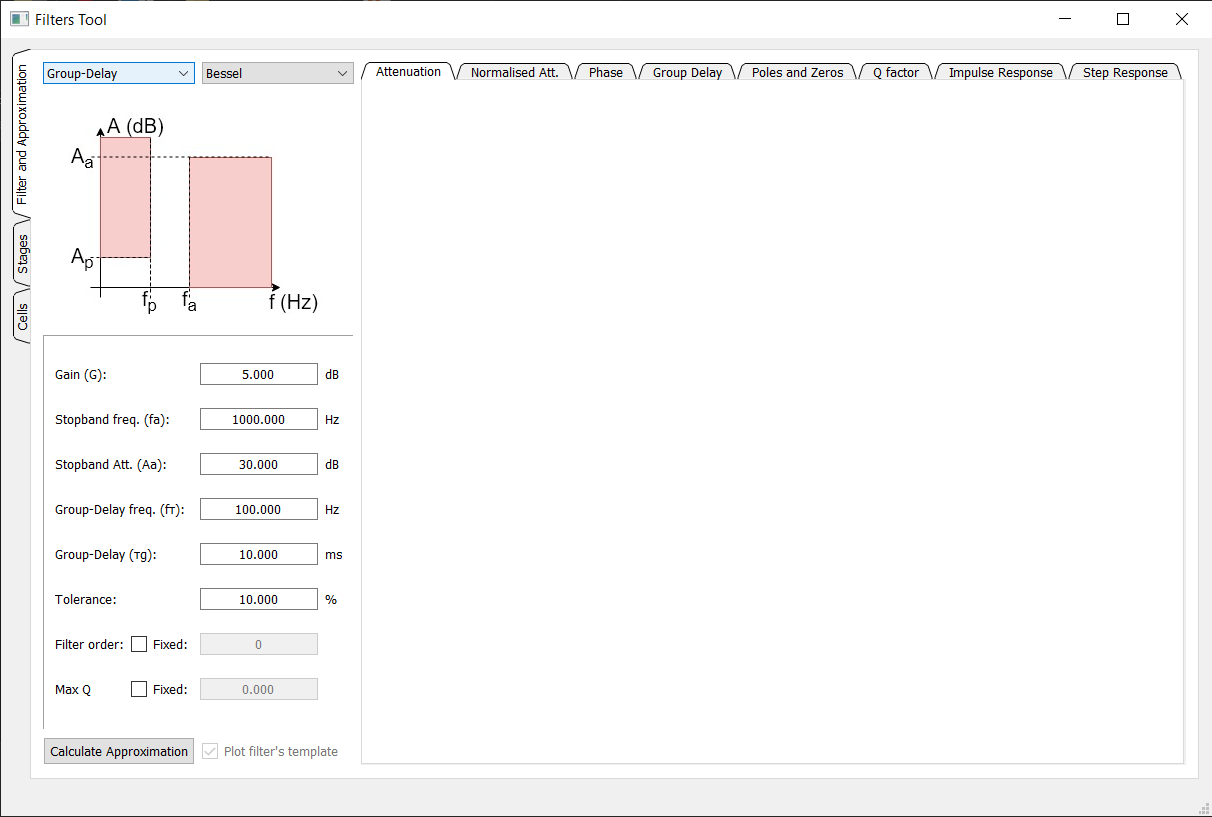
\includegraphics[width=0.8\textwidth]{../Resources/GUI_BASIC}
    \caption{Interfaz gr\'afica b\'asica}
\end{figure} 

\section{Selecci\'on de filtro y plantilla}
En esta etapa es posible elegir tanto los par\'ametros de la plantilla que debe cumplir el filtro, como el tipo de aproximaci\'on a utilizar para el dise\~no.
Se muestra a continuaci\'on una captura de la interfaz, donde se detalla cada una de las secciones de inter\'es. Es importante se\~nalar laclara distini\'on estre filtros que deben cumplir con una plantilla de atenuaci\'on y aquellos cuya plantilla esta dada por el retardo de grupo en la banda de paso.
\begin{figure}[H]
    \centering
    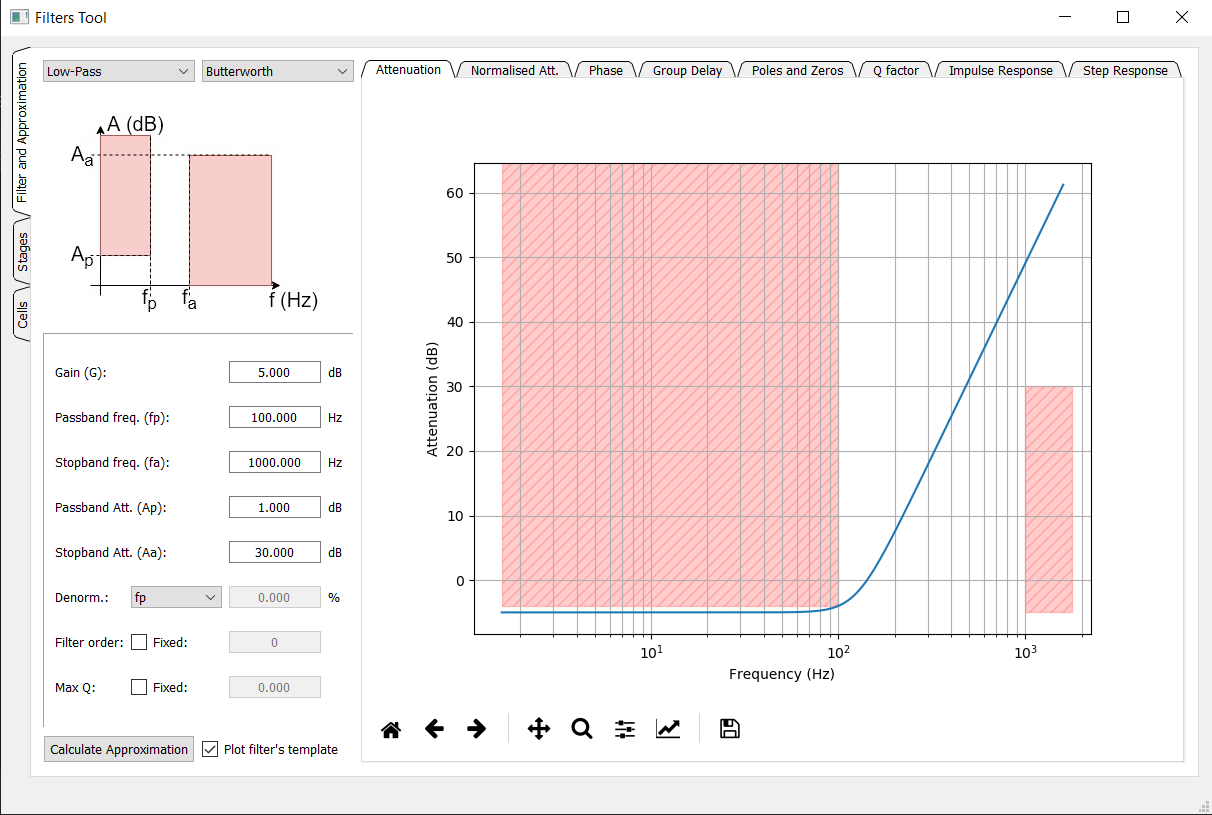
\includegraphics[width=0.8\textwidth]{../Resources/ATT_TEMPLATE}
    \caption{Interfaz gr\'afica la selecci\'on de plantilla. Plantilla de atenuaci\'on}
\end{figure} 
\begin{figure}[H]
    \centering
    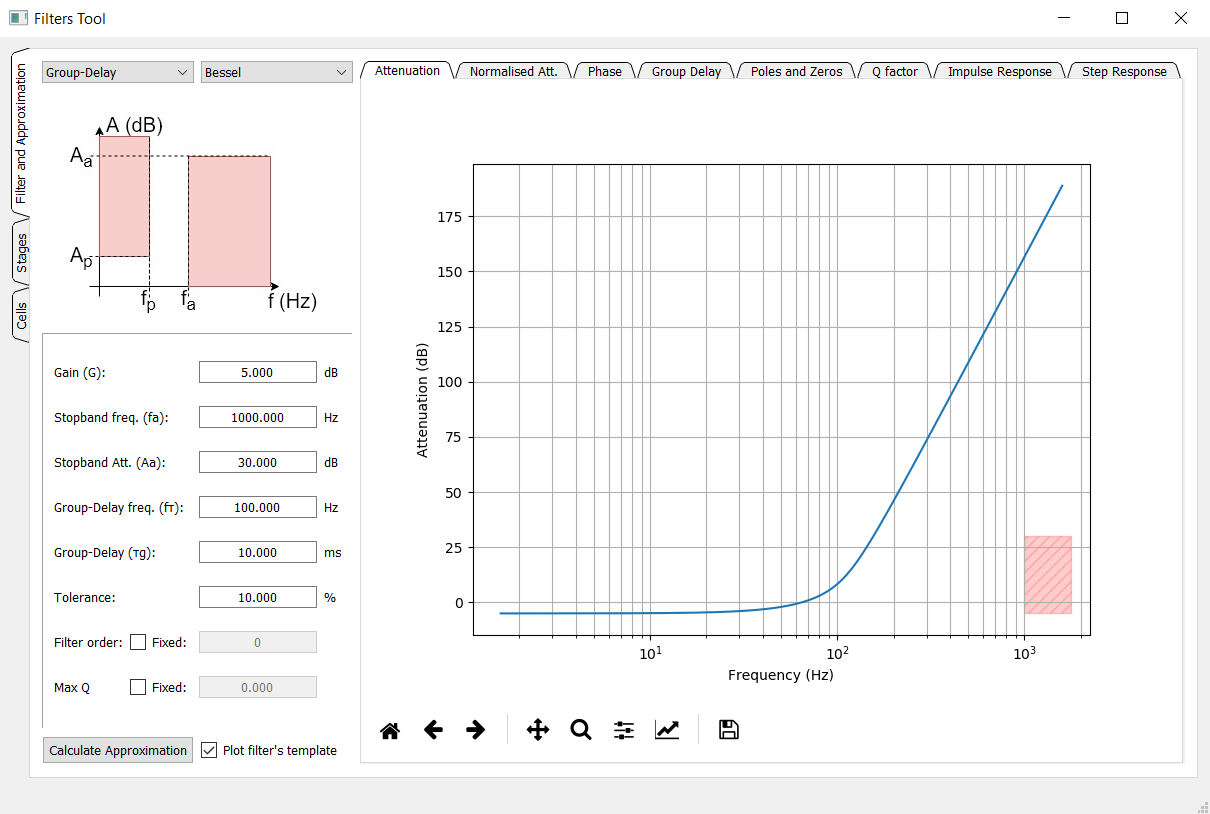
\includegraphics[width=0.8\textwidth]{../Resources/GD_TEMPLATE}
    \caption{Interfaz gr\'afica la selecci\'on de plantilla. Plantilla de atenuaci\'on}
\end{figure} 

\section{Divisi\'on del sistema por etapas de primer y segundo orden}
\section{Implementaci\'on del circuito}
\section{Dise\~no de un filtro paso a paso}
\end{document}